\documentclass[12pt]{article}
\usepackage[a4paper,total={6in,9in}]{geometry}
\usepackage{wrapfig}
\usepackage{graphicx}
\usepackage{amssymb}
\usepackage{mathtools}
\usepackage{listings}
\usepackage{url}
\usepackage{hyperref}
\usepackage{xcolor}

\author{\textbf{Anshuman Singh} \\ \textbf{2018JTM2004}\\ \textbf{2018-19}}
\date{}
\title{\textbf{Assignment-13\\ELP- 718 Telecom Software Laboratory}}

\begin{document}
	\maketitle
	
	\begin{center}
	\noindent \textbf{A report presented for the assignment on\\ Socket Programming in C}
	\vspace{1cm}
	
	\begin{figure}[h]
	\centering
	
\includegraphics[scale=.2]{iitd.jpg}
	
	
	\end{figure}
	\vspace{1.5cm}
	
	\textbf{Bharti School\\of\\Telecommunication Technology and Management\\IIT DELHI, Delhi\\Novembar 12, 2018}
	
	\end{center}
	
	\newpage
	\tableofcontents
	\listoffigures
	\newpage
	
	\section{Problem Statement-1}
	
	
		\subsection{Problem Statement}
		You’ve to design a simple client and server TCP communication using sockets.
		\begin{enumerate}


		\item Server before establishing connection with the client should ask client for credentials.If
		valid (authenticate user\_id and password entered by the client) then allow connection
		otherwise prompt client again for id and password.
		\item After successful authentication, the client sends a string to server and the server change
		the case of each alphabet and send it back to client.
		\item The client take user input from console as to what string has to be sent.The returned
		string is displayed underneath.
		\item The communication continues on as long as server or client don’t close their sockets.
		\item The different stages of TCP communication should be shown with corresponding
		messages as well. You should also display error in case of failures.
		\end{enumerate}		
		
		\subsection{Assumptions}
		
			\begin{itemize}
				\item Credentials are stored in a file named user\_pass.
				\item All processing is done at the server.
			\end{itemize}
		
		\subsection{Algorithm and Implementation~\cite{1}~\cite{2}~\cite{3}}
			\textbf{Server Side:}
			\begin{itemize}
				\item Create a socket file descriptor first.
				\item Specify the address family as IPv4 and IP address as the IP of the system.
			    \item Bind the socket to a port number.
			    \item Listen for connections from the clients.
			    \item Now accept connections from clients and store their socket descriptors.
			    \item Ask for credentials from the client.
			    \item Authenticate or ask again for credentials.
			    \item Create a child process using fork for each new connection.
			    \item Create a function to receive the input string from the user.
			    \item Then call the function written to process the query.
			    \item Return the query and ask again for the next query.
			\end{itemize}
			\textbf{Client Side:}
			\begin{itemize}
				\item Create a socket file descriptor first.
				\item Specify the address family as IPv4 and IP address as the IP of the system.
				\item Bind to the port number on which server is running.
				\item Connect to server using the port number and address family specified.
				\item Provide credentials.
				\item Keep asking for query from user and process it.
				\item Re-enter the query for processing until quit is pressed.
			\end{itemize}			
		\subsection{Flow Chart}
		
			\begin{figure}[h!]
				\centering
				\caption{Flow Chart for Figure 1}
				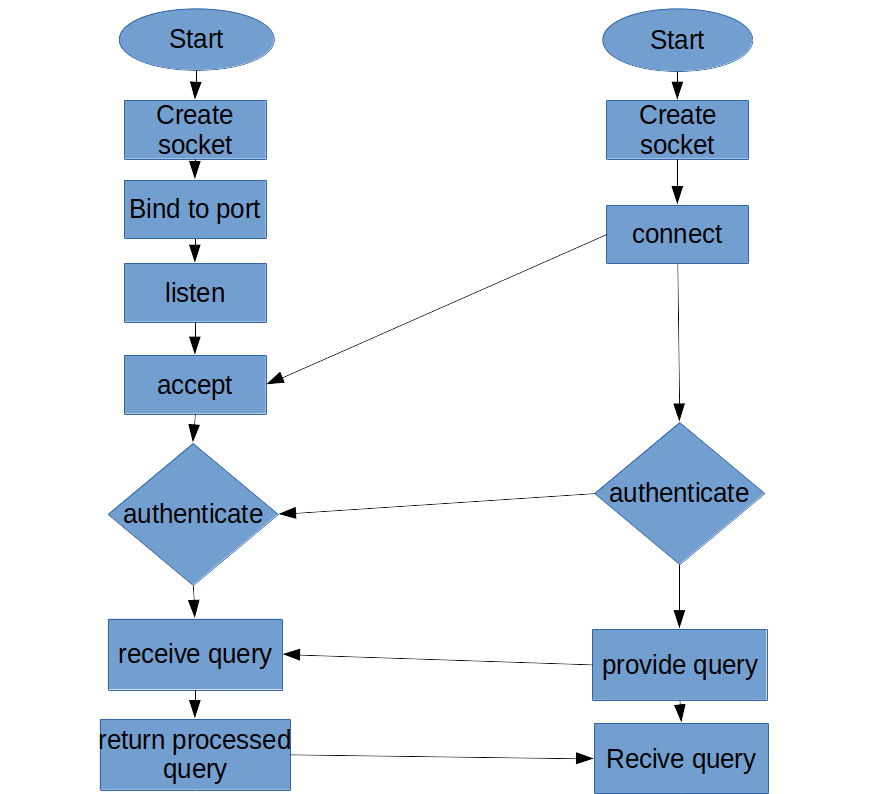
\includegraphics[scale=.4]{flow.png}
			\end{figure}
		
		\subsection{Input and Output Format}
		
			\begin{itemize}
				\item \textbf{Client Interface example(on connection)}:\\
				Please Enter Username: “xyz”
\\
				Please Enter Password: “4567”
\\
				Enter the string: HelLo (if credentials are valid)
\\
				Reply from server : hELlO
\\
				Enter the string :
				\item \textbf{Server Interface example}:\\ 
				Validate the credentials
\\
				String received : HelLo
\\
				Replied string : hELlO
			\end{itemize}
		
		\subsection{Screenshots}
		
			\begin{figure}[h!]
				\centering
				\caption{Terminal Output of Server Assignment 1}
				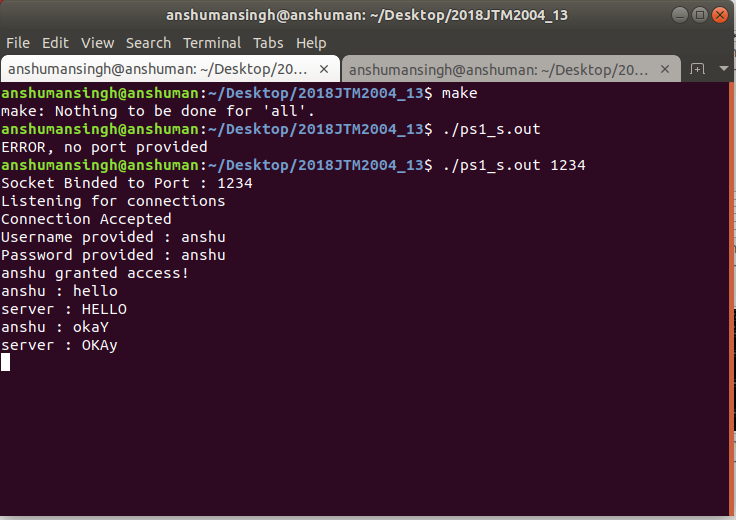
\includegraphics[scale=.6]{ps1_o_1.png}
			\end{figure}
			\begin{figure}[h!]
				\centering
				\caption{Terminal Output of Client Assignment 1}
				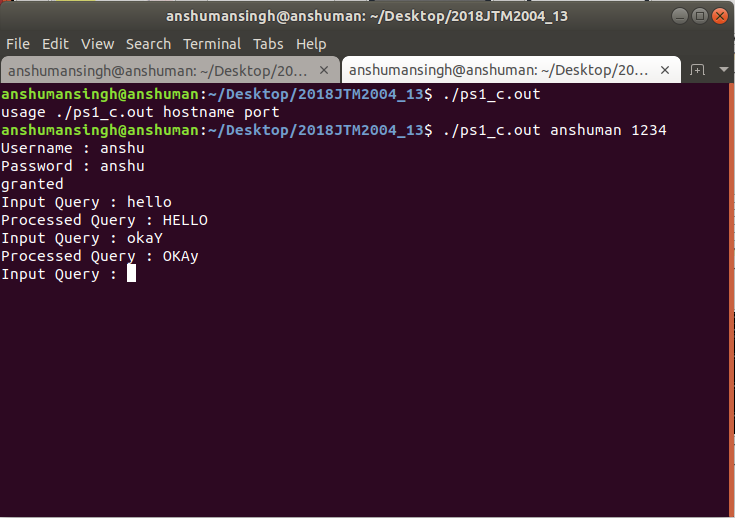
\includegraphics[scale=.6]{ps1_o_2.png}
			\end{figure}

	\section{Problem Statement-2}
	
		\subsection{Problem Statement}
		You have to create a server capable of handling multiple clients up to 5 and ​rejecting more
		than 5 connections ​using TCP communication sockets.Server should work in following phases.
		\begin{enumerate}
		\item Server before establishing connection with the client should ask client for credentials.If
		valid (authenticate user\_id and password entered by the client) then allow connection
		otherwise prompt client again for id and password.
		\item After successful authentication ,conversation should start between clients and
		server.Store the chat history between server and clients in a file “chat.txt” along with the
		timestamp ( containing date and time )adjacent to the chat string.
		\item One message send by a client should be broadcasted to all clients.
		\item Before broadcasting the message server modify the message send by client by adding
		prefix to the message.
				\end{enumerate}
			
		
		\subsection{Assumptions}
		
			\begin{itemize}
				\item Credentials are stored in a file named user\_pass.
				\item Chat history gets stored in a file named chat\_history.
			\end{itemize}
		
		\subsection{Algorithm and Implementation~\cite{1}~\cite{2}~\cite{3}}
			\textbf{Server Side:}
			\begin{itemize}
				\item Create a socket file descriptor first.
				\item Specify the address family as IPv4 and IP address as the IP of the system.
				\item Bind the socket to a port number.
				\item Listen for connections from the clients.
				\item Now accept connections from clients and store their socket descriptors.
				\item Ask for credentials from the client.
				\item Authenticate or ask again for credentials.
				\item Keep checking for data from all clients.
				\item When data is present broadcast it to all the clients along with prefix.
				\item Store the chat history in a file.
				\item When quit is given as input quit the client program.
			\end{itemize}
			\textbf{Client Side:}
			\begin{itemize}
				\item Create a socket file descriptor first.
				\item Specify the address family as IPv4 and IP address as the IP of the system.
				\item Bind to the port number on which server is running.
				\item Connect to server using the port number and address family specified.
				\item Provide credentials.
				\item Enter message to broadcast until quit is given.

			\end{itemize}			
		\newpage
		\subsection{Flow Chart}
		
			\begin{figure}[h!]
				\centering
				\caption{Terminal Output of Server Assignment 2}
				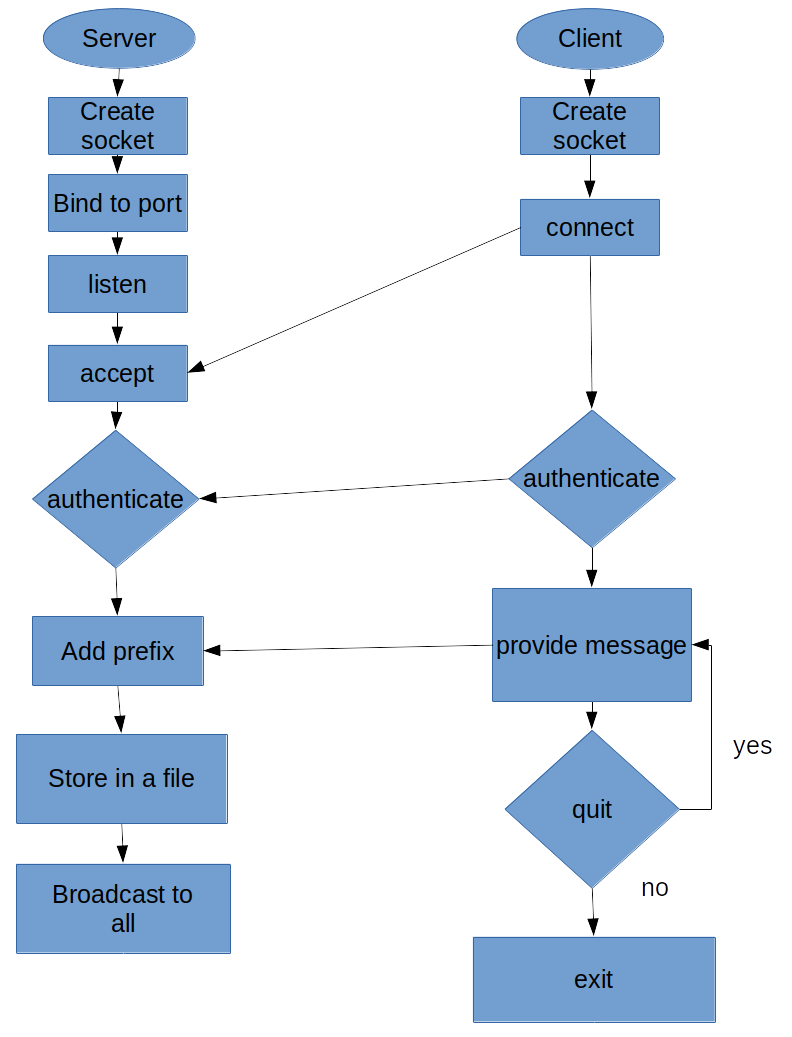
\includegraphics[scale=.55]{flow_2.png}
			\end{figure}
		
		\subsection{Input and Output Format}
			\textbf{Client interface example:}
			\begin{itemize}
				\item Please Enter Username: “abc”
				\item Please Enter Password: “1234”
				\item Received String: Valid/Enter Credentials Again
			 
			\end{itemize}
			\textbf{Server Interface example(on connection):}
			\begin{itemize}
				\item ./server.out xyz\_

				\item  xyz\_ - prefix
				
			\end{itemize}

		\subsection{Screenshots}
			\begin{figure}[h!]
				\centering
				\caption{Terminal Output of Server Assignment 2}
				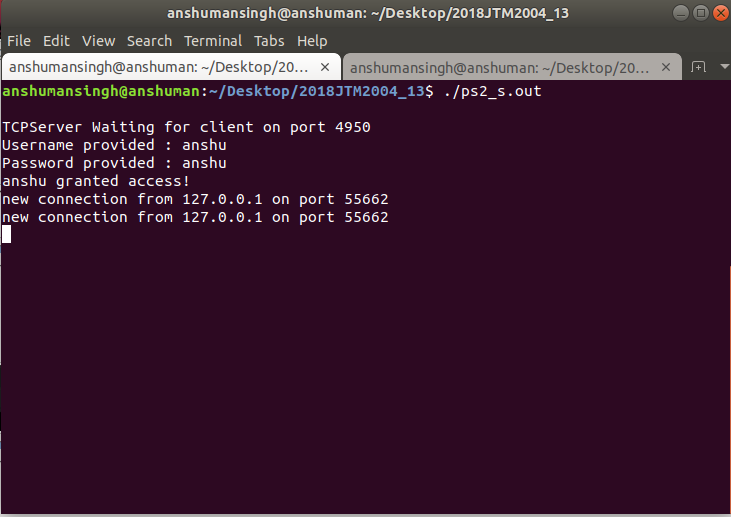
\includegraphics[scale=.55]{ps2_o_1.png}
			\end{figure}
			\begin{figure}[h!]
				\centering
				\caption{Terminal Output of Client Assignment 2}
				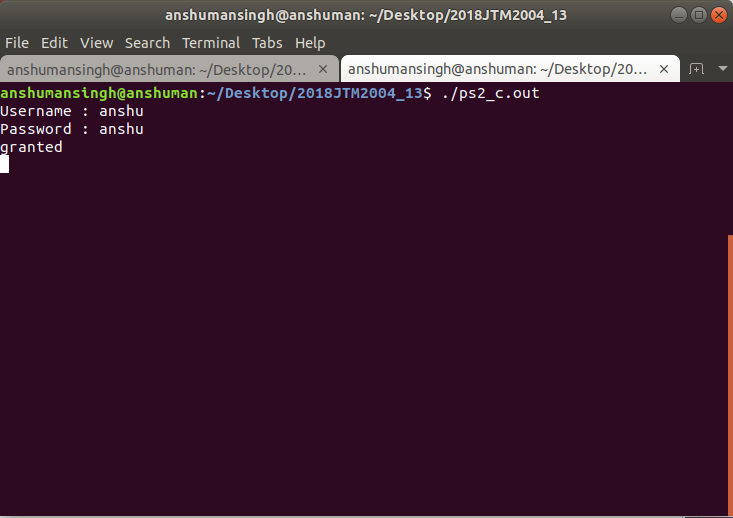
\includegraphics[scale=.55]{ps2_o_2.png}
			\end{figure}
	\newpage
	\section{Appendix}
	
		\definecolor{mygreen}{HTML}{087012}
		\definecolor{mygray}{HTML}{7e7f81}
		\definecolor{mymauve}{HTML}{cb5be2}
		
		\lstset{
			language=C,
			backgroundcolor=\color{white}, 
			basicstyle=\footnotesize,        % size of fonts
			breaklines=true,                 % automatic line breaking
			captionpos=b,                  
			commentstyle=\color{mygreen},    % comment style
			keywordstyle=\color{blue},       % keyword style
			stringstyle=\color{mymauve},     % string literal style
		}
		\subsection{Code for ps1\_s}
			\lstinputlisting[]{ps1_s.c}
		\subsection{Code for ps1\_c}
			\lstinputlisting[]{ps1_c.c}
		\subsection{Code for ps2\_s}
			\lstinputlisting[]{ps2_s.c}
		\subsection{Code for ps2\_c}
			\lstinputlisting[]{ps2_s.c}
		


		\bibliographystyle{plain}
		\bibliography{report.bib}

\end{document}
